\section{Simulated speckle and the comparison to experiment}

\begin{figure}[tbp]
    \begin{center}
    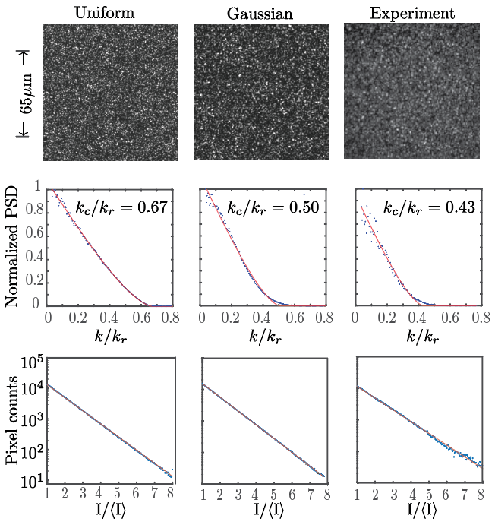
\includegraphics{Chapter4_secs/optical_speckle.pdf}
    \end{center}
    
    \caption{Simulated and measured optical speckle. The columns in the figure correspond to: simulated speckle with uniform laser beam,  simulated speckle from a Gaussian laser beam and measured speckle. In each column, the first row shows the intensity of the optical speckle field. The second row shows the PSD of the intensity shown in the first row (symbols).  The red curve shows a fit of Eq.~(\ref{psd_image}) to the data, along with the resulting $k_c$. The third row histograms the  intensity from the first row. }
    \label{fig:Optical speckle}
\end{figure}

Having now fully set the stage for understanding and creating speckle laser beams, we turn to laboratory confirmation of key prediction of these models relevant to cold atom experiment: the field-field correlation length $C_E$ and the distribution of intensities $P(I)$.

In our lab, we directed a collimated laser beam (waist $w\approx25\ {\rm mm}$) through a diffuser (divergence angle $\theta_d = 0.5^\circ$, and aperture $D=20\ {\rm mm}$) focused immediately by a lens (focal length $f = 30 {\rm mm}$) as depicted in Fig.~(\ref{fig:speckle1}) and quantified the optical speckle formed at the focal plane.  We then imaged the optical speckle onto a charge coupled device (CCD) camera with Keplerian telescope with magnification $M=46$.  The CCD's $1024 \times 1280$ array of $4.8\ \mu {\rm m}$ pixels gave a $100\ \mu{\rm m} \times 130\ \mu{\rm m}$ magnified field of view with $0.1\ \mu {\rm m}$ pixels.

Our analytic results for $C_E$ are valid in the Gaussian beam limit ( $w\ll D$) or uniform illumination limit ($w\gg D$).  Because our experiment has $w\approx D$, we numerically simulated the optical speckle to compare with our measurements and both models.

For the numerical simulation, the desired optical speckle field $E_{i,j}$ is represented by a $1024 \times 1280$ array at the focal point of the lens.  We use the optical Fourier transform property of lenses to compute this efficiently, whereby the field a focal distance beyond the lens is related to the Fourier transform of the field a focal distance prior to the lens (which we will term the Fourier plane).  An important aspect of this method is that the $0.1\ \mu {\rm m}$ grid spacing in the focal plane transforms to a $1.5\ {\rm mm}$ grid spacing in the Fourier plane.

Our simulation progresses as follows.  (1) We first initialize $E_{i,j}(z=0)$ to the field of either a uniform field or a Gaussian beam.  (2) We then imprint random phases on each point~\footnote{The grid size is much larger than the correlation length of the diffuser, so the imprinted phase at each grid point is uncorrelated with all other points.}.  (3) We set the field outside our physical aperture to zero.  (4) Then we back-propagate the field to the Fourier plane and take the Fourier transform to obtain the field at the focal plane.

Fig.~(\ref{fig:Optical speckle}) compares our measured speckle with numerics and our analytic model; the three columns depict: the case of a uniformly illuminated aperture, Gaussian illumination, and experiment.   The top row shows that intensity at the focal plane is qualitatively similar for all three cases. In the middle row, the PSD (computed from the intensity in the top row, and plotted by blue symbols), highlights the differences.  In each case, we fit Eq.~(\ref{psd_image}) the PSD and extract $k_c$ from the fits (red curves).  Because  Eq.~(\ref{psd_image}) was derived for a uniformly illuminated aperture it provides a good fit to the uniform illumination case but deviates at large $k$ for Gaussian illumination and experiment.  In contrast, the numerics for Gaussian illumination and the experiment are indistinguishable.  
% In the numerical simulation, we account for the $20{\rm mm}$ clear aperture of the lenses and diffuser. In the uniform case, our analytical model calculates $k_c = 0.62k_r$ and the numerically calculated PSD agrees with Eq.~(\ref{psd_image}) very well. 
In the bottom row, we histogram the intensity distribution and verify that in all three cases we recover the expected exponential fall-off.